\chapter{Results and Discussions}

%%%%%%%%%%%%%%%%%%%%%%%%%%%%%%%%%%%%%%%%%%%%%%%%%%%%%%%%%%%%%%%%%%%%%%%%%%%%%%%%%%%%
% SECTION: Software tests
%%%%%%%%%%%%%%%%%%%%%%%%%%%%%%%%%%%%%%%%%%%%%%%%%%%%%%%%%%%%%%%%%%%%%%%%%%%%%%%%%%%%
\section{Software Tests}
\subsection{Tests outcome}
\begin{table}[h!]
	\centering
	\caption{Unit and Integration test outcome.}
	\label{table:software_test}
	\begin{tabular}{cccc}
		\hline
		\hline
		\toprule
		\textbf{Hardware} & \textbf{Unit test} & \textbf{Outcome} & \textbf{Coverage estimation}\\
		\bottomrule
		\toprule
		\multirow{3}{*}{internal RTC} & test\_clock\_date & Pass & \multirow{3}{*}{33.33\%}\\
		& test\_clock\_time & Pass &\\
		& test\_clock\_alarm & Pass &\\
		\midrule
		external RTC & test\_rtc\_clock & Pass & 47.1\%\\
		\midrule
		\multirow{3}{*}{queue} & test\_queue\_create & Pass & \multirow{3}{*}{44.44\%}\\
		& test\_queue\_enqueue & Pass &\\
		& test\_queue\_dequeue & Pass &\\
		\midrule
		\multirow{3}{*}{eeprom} & test\_eeprom\_write\_read & Pass & \multirow{3}{*}{66.67\%}\\
		& test\_eeprom\_write4B\_read4B & Pass &\\
		& test\_eeprom\_writeNB\_readNB & Pass &\\
		\midrule
		\multirow{2}{*}{alarm} & test\_alarm\_address & Pass & \multirow{2}{*}{66.67\%}\\
		& test\_alarm\_save\_load & Pass &\\ 
		\bottomrule
		\hline
		\hline
	\end{tabular}
\end{table}

\subsection{Insight on the software tests}


%%%%%%%%%%%%%%%%%%%%%%%%%%%%%%%%%%%%%%%%%%%%%%%%%%%%%%%%%%%%%%%%%%%%%%%%%%%%%%%%%%%%
% SECTION: Hardware module tests
%%%%%%%%%%%%%%%%%%%%%%%%%%%%%%%%%%%%%%%%%%%%%%%%%%%%%%%%%%%%%%%%%%%%%%%%%%%%%%%%%%%%
\section{Hardware module tests}
\subsection{Test results}
\subsubsection{DS1307}
\subsubsection{25LC640}
\subsubsection{HC-06}
\subsubsection{NX4024T032\_001}
\subsubsection{MAX7221}
\subsection{Discussions}

%%%%%%%%%%%%%%%%%%%%%%%%%%%%%%%%%%%%%%%%%%%%%%%%%%%%%%%%%%%%%%%%%%%%%%%%%%%%%%%%%%%%
% SECTION: Ring 
%%%%%%%%%%%%%%%%%%%%%%%%%%%%%%%%%%%%%%%%%%%%%%%%%%%%%%%%%%%%%%%%%%%%%%%%%%%%%%%%%%%%
\section{Ring experiments}

\subsection{Current drawn by the Ring}
\subsubsection{Experimental results}

\begin{table}[h!]
	\centering
	\caption{Current drawn by a one neopixel per colour at different brightness levels. The white colour is obtain by turning the red, green and blue LEDs on at the same brightness.}
	\label{table:current_one_pixel}
	\begin{tabular}{ccccc}
		\hline
		\hline
		\toprule
		\multirow{2}{*}{\textbf{Brightness (\%)}} & \multicolumn{4}{c}{\textbf{Current (mA)}}\\
		& \textbf{Red} & \textbf{Green} & \textbf{Blue} & \textbf{White} \\
		\bottomrule
		\toprule
		0	&	3	&	3	&	3	&	3	\\
		10	&	4	&	4	&	4	&	5	\\
		20	&	5	&	5	&	5	&	9	\\
		30	&	7	&	7	&	6	&	13	\\
		40	&	8	&	8	&	8	&	17	\\
		50	&	10	&	10	&	9	&	22	\\
		60	&	11	&	11	&	11	&	26	\\
		70	&	13	&	12	&	12	&	30	\\
		80	&	14	&	14	&	13	&	34	\\
		90	&	15	&	15	&	15	&	38	\\
		100	&	17	&	17	&	16	&	42	\\
		\bottomrule
		\hline
		\hline
	\end{tabular}
\end{table}

\begin{table}[h!]
	\centering
	\caption{Current drawn by the neopixels in idle mode. The idle mode is defined as the state of the of the neopixel when no light is emitted.}
	\label{table:current_idle}
	\begin{tabular}{cc}
		\hline
		\hline
		\toprule
		\textbf{Number of neopixels} & \textbf{Current (mA)}\\
		\bottomrule
		\toprule
		0	&	89	\\
		10	&	89	\\
		25	&	90	\\
		50	&	92	\\
		90	&	95	\\
		120	&	97	\\
		150	&	99	\\
		180	&	101	\\
		\bottomrule
		\hline
		\hline
	\end{tabular}
\end{table}


\begin{table}[h!]
	\centering
	\caption{Current drawn by all 180 neopixels on the Ring at different brightness levels.}
	\label{table:current_180_neopixels}
	\begin{tabular}{ccccc}
		\hline
		\hline
		\toprule
		\multirow{2}{*}{\textbf{Brightness (\%)}} & \multicolumn{4}{c}{\textbf{Current (A)}}\\
		& \multicolumn{3}{c}{\textbf{Readings}} & \textbf{Average} \\
		\bottomrule
		\toprule
		0	&	0.120	&	0.120	&	0.120	&	0.120	\\
		10	&	0.510	&	0.510	&	0.500	&	0.507	\\
		20	&	1.250	&	1.230	&	1.220	&	1.233	\\
		30	&	2.000	&	1.980	&	1.970	&	1.983	\\
		40	&	2.730	&	2.690	&	2.680	&	2.700	\\
		50	&	3.480	&	3.430	&	3.410	&	3.440	\\
		60	&	4.890	&	4.120	&	4.110	&	4.373	\\
		70	&	4.910	&	4.840	&	4.830	&	4.860	\\
		80	&	5.600	&	5.530	&	5.510	&	5.547	\\
		90	&	6.320	&	6.240	&	6.220	&	6.260	\\
		100	&	7.020	&	6.910	&	6.890	&	6.940	\\
		\bottomrule
		\hline
		\hline
	\end{tabular}
\end{table}

\begin{figure}[ht]
	\centering
	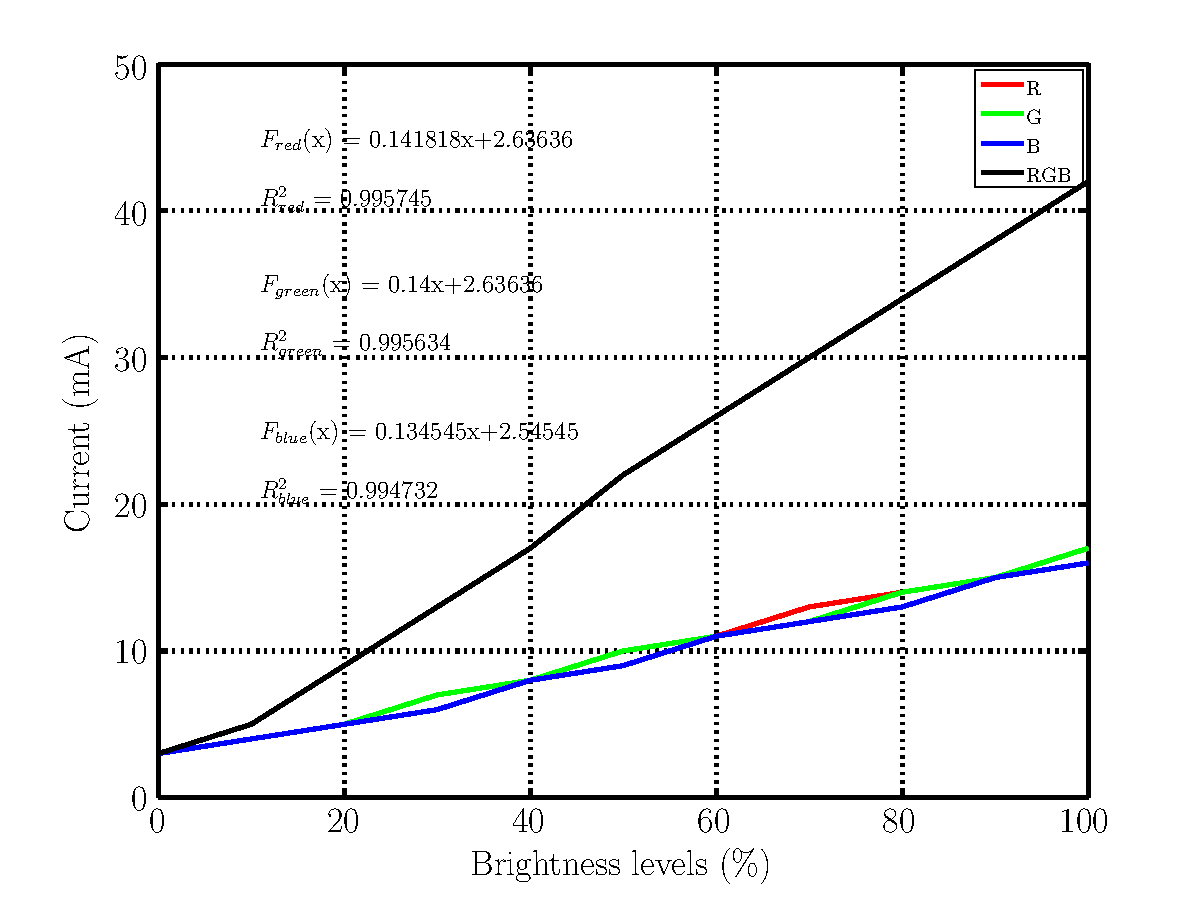
\includegraphics[scale=0.6]{current_one_pixel.pdf}
	\caption{}
	\label{fig:current_one_pixel}
\end{figure}
\begin{figure}[ht]
	\centering
	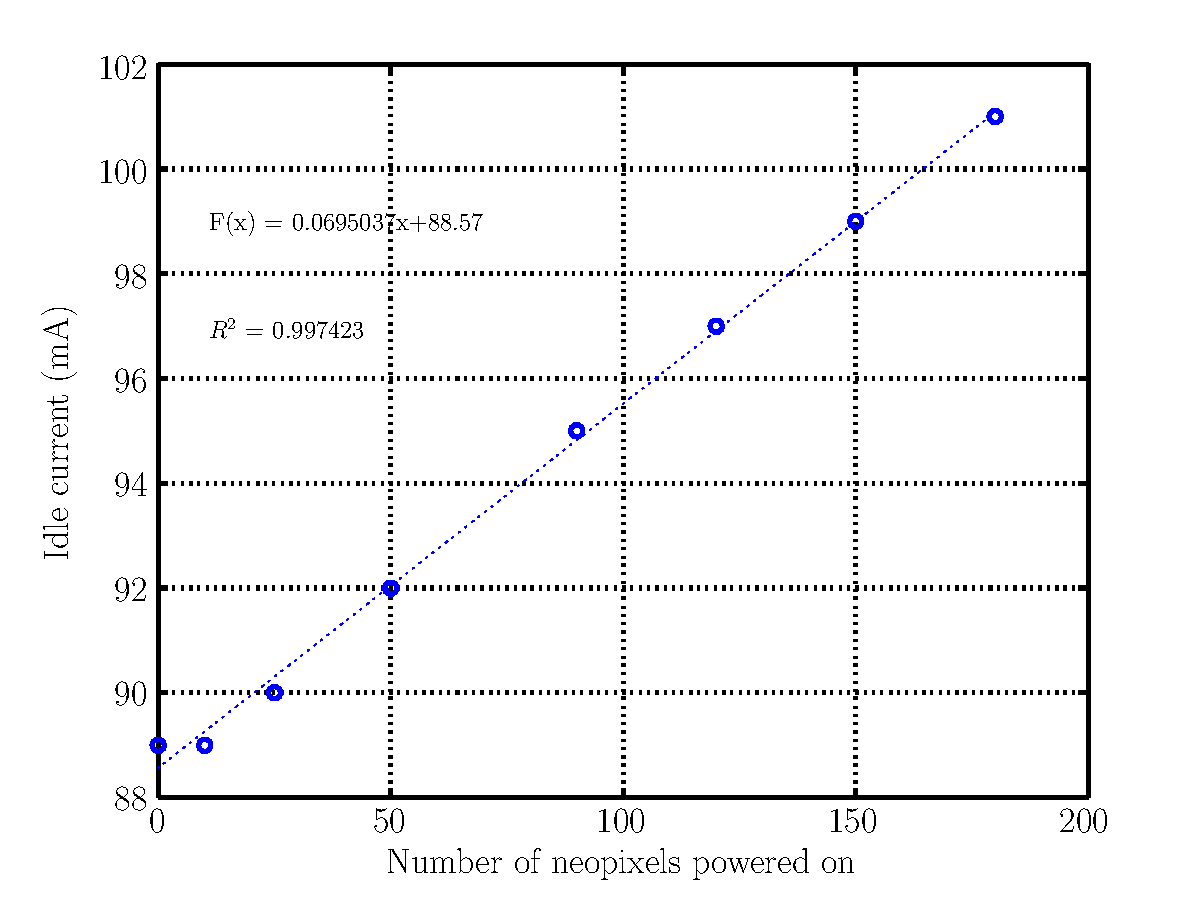
\includegraphics[scale=0.6]{current_idle.pdf}
	\caption{}
	\label{fig:current_idle}
\end{figure}
\begin{figure}[ht]
	\centering
	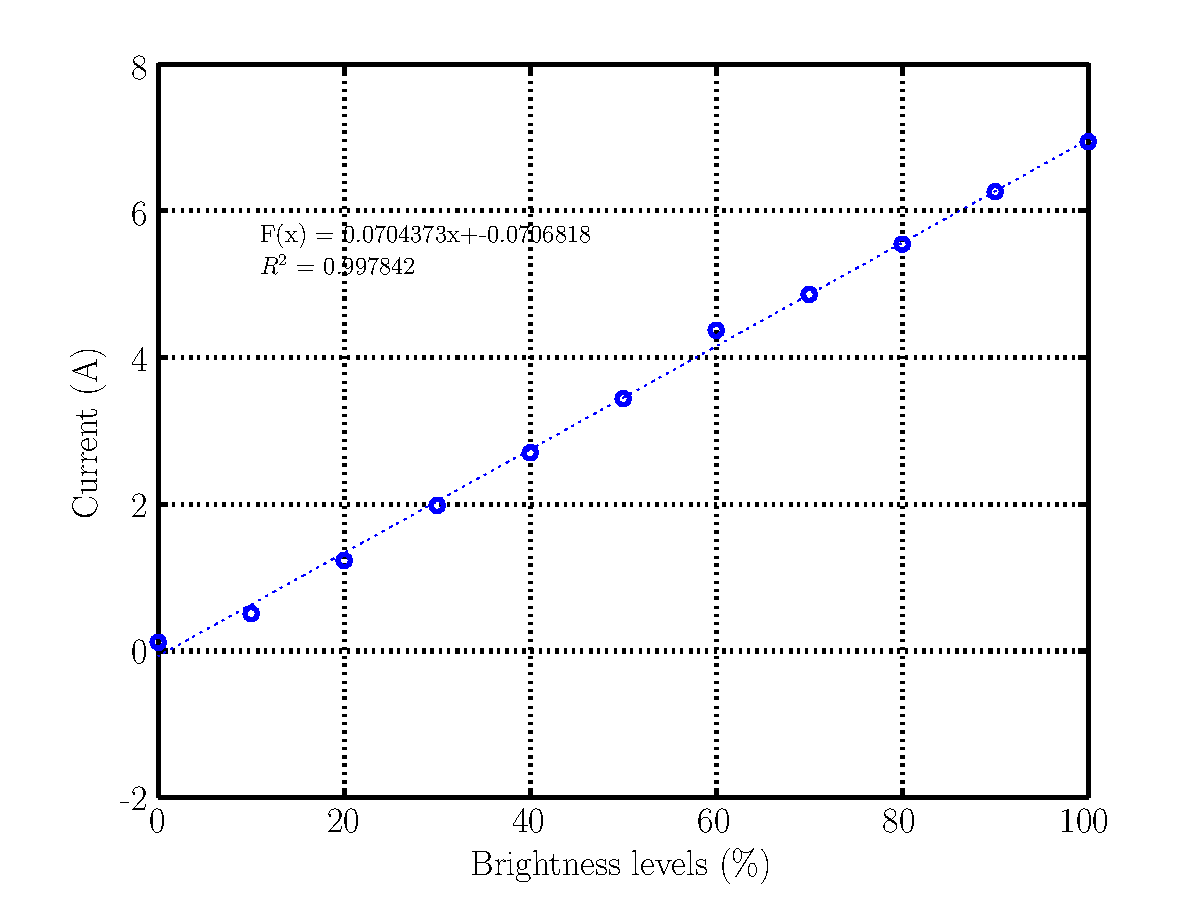
\includegraphics[scale=0.6]{current_180_neopixels.pdf}
	\caption{}
	\label{fig:current_180_neopixels}
\end{figure}

\subsubsection{Discussion}

\subsection{Ring temperature by the Ring}
\subsubsection{Experimental results}

\begin{table}[h!]
	\centering
	\caption{Current drawn by the neopixels in idle mode. The idle mode is defined as the state of the of the neopixel when no light is emitted.}
	\label{table:temperature_ring}
	\begin{tabular}{cc}
		\hline
		\hline
		\toprule
		\textbf{Current (A)} & \textbf{Temperature ($^oC$)}\\
		\bottomrule
		\toprule
		0.09	&	2.176	\\
		0.49	&	6.417	\\
		1.24	&	11.750	\\
		1.95	&	17.667	\\
		3.38	&	28.083	\\
		4.1		&	29.667	\\
		5.35	&	39.000	\\
		6		&	43.091	\\
		6.55	&	44.750	\\
		\bottomrule
		\hline
		\hline
	\end{tabular}
\end{table}
\begin{figure}[ht]
	\centering
	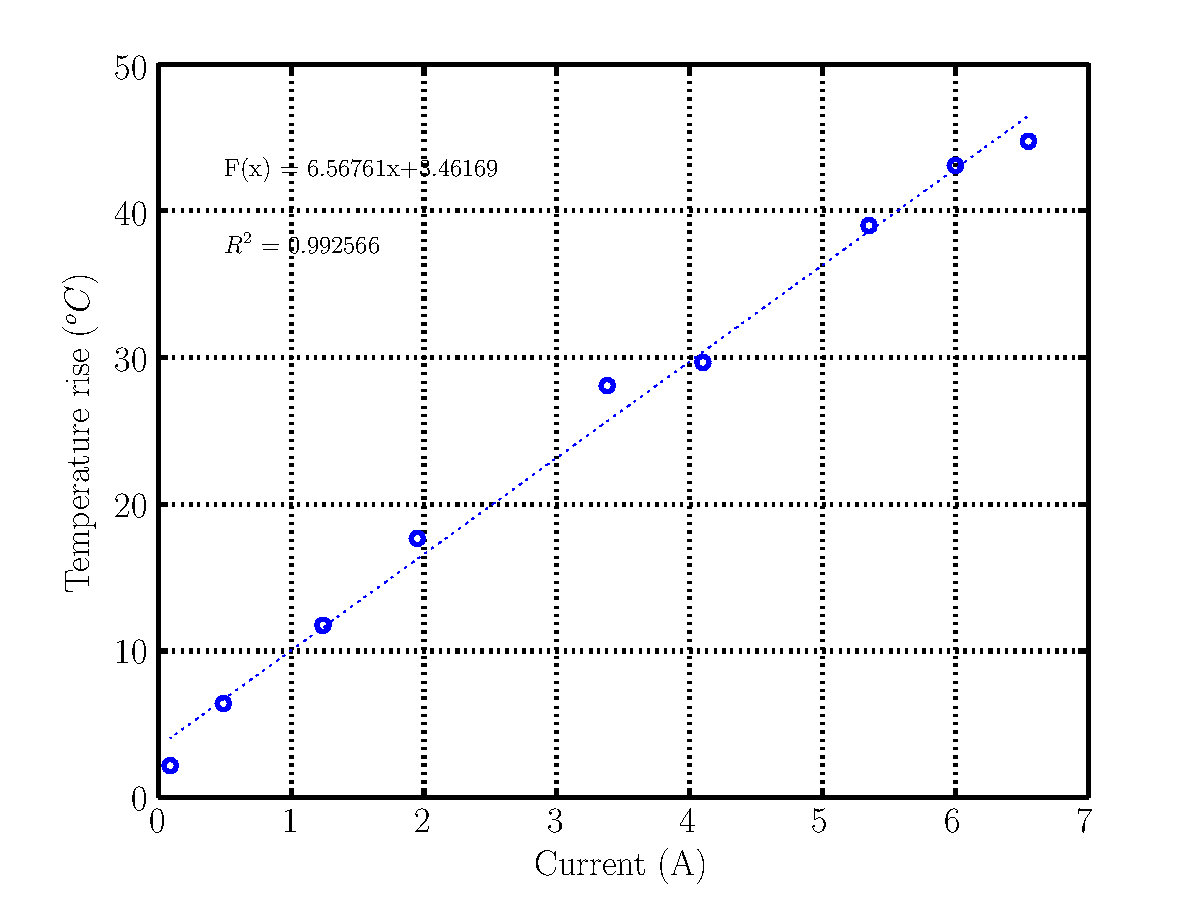
\includegraphics[scale=0.6]{temperature_ring.pdf}
	\caption{}
	\label{fig:temperature_ring}
\end{figure}

\subsubsection{Discussion}

\subsection{Illuminance produced by the Ring}
\subsubsection{Experimental results}

\begin{table}[h!]
	\centering
	\caption{Ring's blue LED illuminance at full brightness per distance and angular section to the Ring.}
	\label{table:illuminance_blue}
	\begin{tabular}{ccccc}
		\hline
		\hline
		\toprule
		\multirow{2}{*}{\textbf{Distance (cm)}} & \multicolumn{4}{c}{\textbf{Angle (deg)}}\\
		& 0 & 30 & 60 & 90 \\
		\bottomrule
		\toprule
		20	&	6420	&	5950	&	5310	&	1998	\\
		30	&	4910	&	3770	&	3302	&	547		\\
		40	&	2507	&	2354	&	1657	&	149		\\
		50	&	1820	&	1620	&	1219	&	110		\\
		60	&	1375	&	1227	&	892		&	60		\\
		70	&	1012	&	943		&	691		&	55		\\
		80	&	810		&	785		&	547		&	43		\\
		90	&	667		&	607		&	420		&	35		\\
		100	&	557		&	500		&	353		&	30		\\
		\bottomrule
		\hline
		\hline
	\end{tabular}
\end{table}
\begin{figure}[ht]
	\centering
	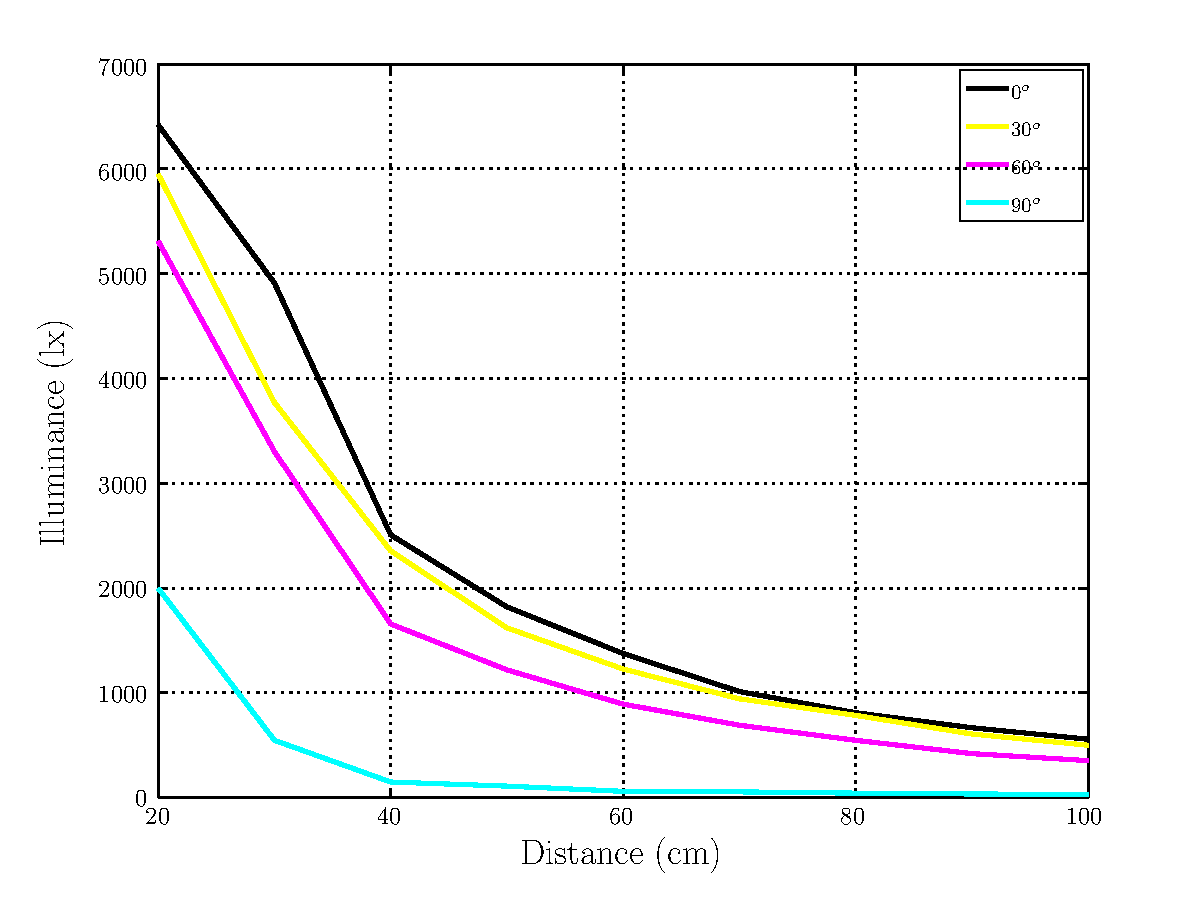
\includegraphics[scale=0.6]{illuminance_blue.pdf}
	\caption{}
	\label{fig:illuminance_blue}
\end{figure}

\begin{table}[h!]
	\centering
	\caption{Relationship between the coefficient of decadence of the Ring illuminance and the distance to the Ring.}
	\label{table:illuminance_distance}
	\begin{tabular}{cccccccc}
		\hline
		\hline
		\toprule
		\multirow{2}{*}{\textbf{Distance (cm)}} & \multicolumn{5}{c}{\textbf{Brightness (\%)}} & \multirow{2}{*}{\textbf{Average}} & \multirow{2}{*}{\textbf{Std dev}}\\
		& 10 & 30 & 50 & 80 & 90 &&\\
		\bottomrule
		\toprule
		20	&	1.00	&	1.00	&	1.00	&	1.00	&	1.00	&	1.00	&	0.00	\\
		30	&	0.68	&	0.63	&	0.65	&	0.65	&	0.59	&	0.64	&	0.03	\\
		40	&	0.44	&	0.40	&	0.44	&	0.41	&	0.36	&	0.41	&	0.03	\\
		50	&	0.31	&	0.29	&	0.31	&	0.28	&	0.27	&	0.29	&	0.02	\\
		60	&	0.23	&	0.20	&	0.23	&	0.22	&	0.20	&	0.22	&	0.01	\\
		70	&	0.18	&	0.15	&	0.18	&	0.17	&	0.15	&	0.17	&	0.01	\\
		80	&	0.14	&	0.13	&	0.14	&	0.13	&	0.12	&	0.13	&	0.01	\\
		90	&	0.12	&	0.10	&	0.11	&	0.13	&	0.10	&	0.11	&	0.01	\\
		100	&	0.10	&	0.08	&	0.09	&	0.09	&	0.08	&	0.09	&	0.01	\\
		\bottomrule
		\hline
		\hline
	\end{tabular}
\end{table}
\begin{figure}[ht]
	\centering
	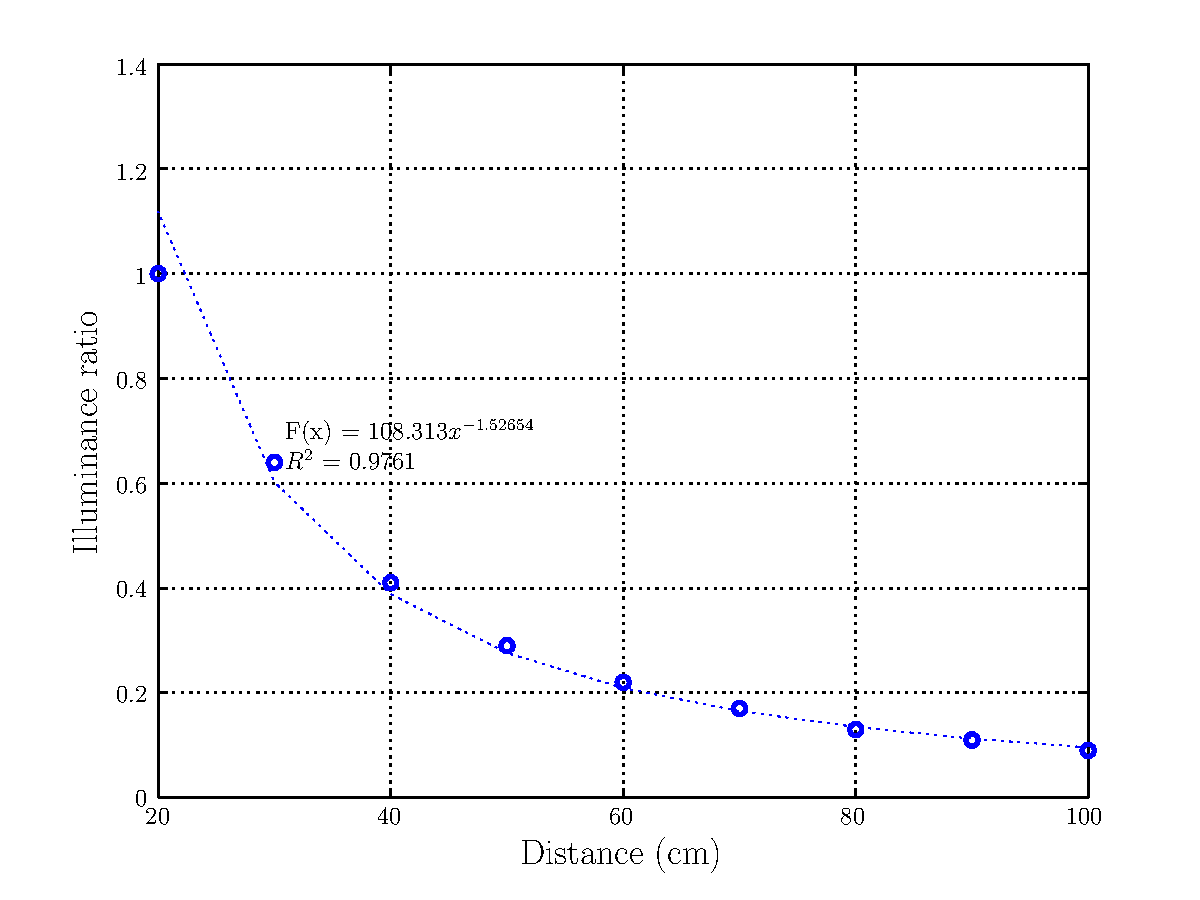
\includegraphics[scale=0.6]{illuminance_distance.pdf}
	\caption{}
	\label{fig:illuminance_distance}
\end{figure}

\begin{table}[h!]
	\centering
	\caption{Relationship between the Ring illuminance and the angle to the normal of the Ring surface.}
	\label{table:illuminance_angle}
	\begin{tabular}{cccccccc}
		\hline
		\hline
		\toprule
		\multirow{2}{*}{\textbf{Angle (cm)}} & \multicolumn{5}{c}{\textbf{Distance (cm)}} & \multirow{2}{*}{\textbf{Average}} & \multirow{2}{*}{\textbf{Std dev}}\\
		& 20 & 30 & 50 & 80 & 100 &&\\
		\bottomrule
		\toprule
		0	&	1.00	&	1.00	&	1.00	&	1.00	&	1.00	&	1.00	&	0.00	\\
		30	&	0.88	&	0.89	&	0.53	&	0.94	&	0.90	&	0.83	&	0.16	\\
		60	&	0.75	&	0.70	&	0.65	&	0.64	&	0.64	&	0.68	&	0.05	\\
		90	&	0.20	&	0.16	&	0.09	&	0.06	&	0.05	&	0.11	&	0.07	\\
		\bottomrule
		\hline
		\hline
	\end{tabular}
\end{table}
\begin{figure}[ht]
	\centering
	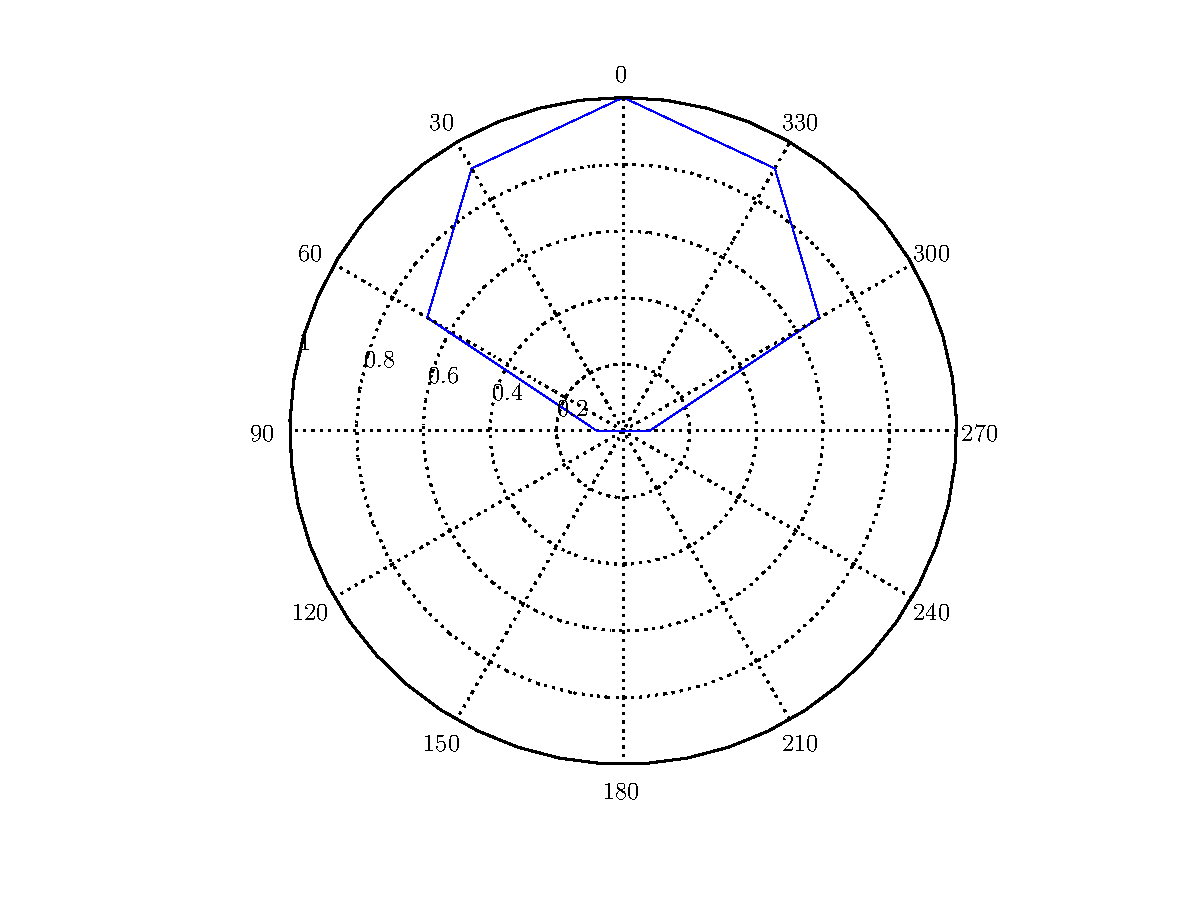
\includegraphics[scale=0.6]{illuminance_angle.pdf}
	\caption{}
	\label{fig:illuminance_angle}
\end{figure}


\subsubsection{Discussion}